\chapter{مدل ریاضی}
\label{ch:fasl2}

روش‌های متعددی برای مدل‌کردن جریان سیالات در محیط متخلخل وجود دارند. مدل پیچیده‌تر معمولاً منجر به جواب‌های دقیق‌تری می‌شود، اما پیاده‌سازی و حل عددی آن دشوارتر خواهد بود. به علاوه مدل‌های پیچیده نیاز به اندازه‌گیری پارامتر‌های تجربی بیشتری دارند که ممکن است اندازه‌گیری آن‌ها همیشه عملی نباشد. لذا در انتخاب مدل مناسب باید به همهٔ این عوامل توجه کرد. همانطور که در بخش \ref{ch:fasl1} عنوان شد، در این پروژه از مدل جریان دوفازی غیرقابل امتزاج و تراکم‌ناپذیر استفاده خواهیم کرد. در این بخش ابتدا مفاهیم کلی استفاده شده در این مدل معرفی خواهند شد. در ادامه نحوه مدلسازی ترک‌ها به روش گسسته بیان می‌شوند. لازم به ذکر است که مطالب این فصل مگر در مواردی خاص که به صورت صریح اشاره شده‌اند، از \cite{basthabil,bear} انتخاب شده‌اند.

%----------------------------------------------------------------------------------------ی
%----------------------------------------------------------------------------------------ی
%                                       قسمت اوّل : محیط متخلخل
%----------------------------------------------------------------------------------------ی
%----------------------------------------------------------------------------------------ی

\section{محیط متخلخل}
محیط متخلخل، جسمی است که از یک جامد تکه‌تکه به نام ماتریس و فضای خالی تشکیل شده است. فضای خالی توسط یک یا چند سیال پر می‌شود. خاک، سنگ‌های آهکی، نان، ریه و کلیه‌ها همگی نوعی محیط متخلخل محسوب می‌شوند. بدیهتاً محیط متخلخل مورد نظر در این پروژه سنگ مخازن نفتی می‌باشد.در محیط متخلخل \text‌سیاه{فاز}\footnote{Phase} و \text‌سیاه{جزء}\footnote{Component} دو تعریف اساسی محسوب می‌شوند. فاز قسمتی از سیستم است که با مرز مشخصی از دیگر قسمت‌ها جدا شده است. برای مثال آب، روغن و ماتریس می‌توانند هر کدام یک فاز را تشکیل دهند در حالی که آب و نمک حل شده در آن فقط یک فاز هستند. جزء قسمتی از یک فاز است که ترکیب شیمیایی متمایزی نسبت به دیگر قسمت‌های آن فاز داشته باشد. لذا مثال آب و نمک عنوان شده یک فاز و دو جزء خواهد بود. لازم به ذکر است که در یک مدل خاص برای ساده‌سازی امکان دارد که وجود چندین جزء داخل یک فاز با یک جزء معادل مدل شود. دو فاز قابل \text‌سیاه{امتزاج} هستند در صورتی که ماده بتواند بین مرز آن‌ها تبادل شود. چند مدل استفاده شده برای جریان در محیط متخلخل با توجه به تعاریف بالا در جدول \ref{tab:2model} دسته‌بندی شده‌اند (فاز سنگ در نظر نگرفته نشده‌است).

\begin{table}
\centering
\caption{مقایسه چند مدل جریان در محیط متخلخل از نظر فازها و اجزاء}
\label{tab:2model}
\begin{tabular}{|c|c|c|c|}
\hline
ردیف &نام مدل &مثالی برای فاز‌ها &اجزاء حاضر  \\
\hline
۱ &تک‌فاز چند‌جزء &برای مثال آب  &انواع رسوبات و آب \\
۲ &دو‌فاز بدون امتزاج &آب و روغن &آب و روغن  \\
۳ &نفت‌سیاه &آب، نفت و گاز &آب و نفت‌گاز(یک جزء)  \\
۴ &ترکیبی &آب، نفت و گاز &آب، انواع هیدروکربن‌ها و گاز‌های دیگر  \\
\hline
\end{tabular}
\end{table}

محیط پیوسته می‌تواند در مقیاس‌های متفاوتی مطالعه شود. حالت پرکاربردی که در شبیه‌سازی مخازن نفتی استفاده می‌شود مقیاس ماکروسکوپیک  نام دارد. در این مقیاس ابعادی که با آن‌ها سر و کار داریم در حدود ده‌ها متر هستند.
\begin{figure}
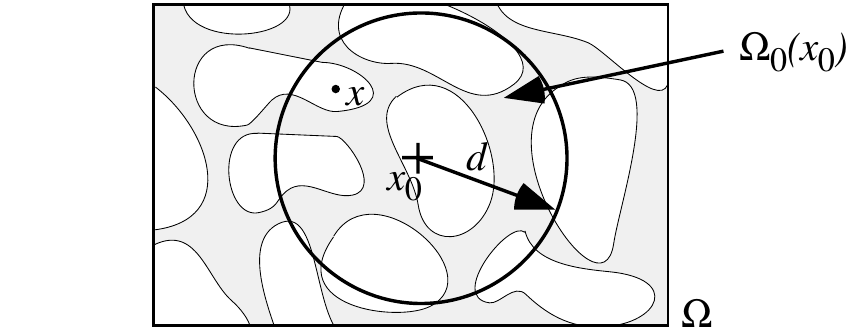
\includegraphics[width=0.6\textwidth,center]{model-rev1}
\caption{شماتیک حجم نماینده}
\label{fig:2rev1}
\end{figure}


 برای تعریف خواصی مثل چگالی، لزجت و \dots‌خ{} در  مقیاس ماکروسکوپیک، باید مقدار متناظر این خاصیت در یک حجم نماینده\footnote{Representetive Elementary Volume - REV} در اطراف هر نقطه متوسط‌گیری شود. در شکل \ref{fig:2rev1} به صورت شماتیک حجم نماینده اطراف نقطه $x_0$ با نام
 $\Omega_0(x_0)$
 و شعاع $d_0$ نمایش داده شده است. در مقیاس ماکروسکوپیک، نقطه‌ای مثل $x_0$ نماینده تمام نقاط داخل 
 $\Omega_0(x_0)$
(مثلاّ $x$) خواهد بود. در صورتی که نحوه تغییرات خواص متوسط (برای مثال تخلخل $\phi$) نسبت به شعاع حجم نماینده روندی مانند شکل \ref{fig:2rev2}  داشته باشد و خواص ماکروسکوپیک به ازای بازه‌ای از شعاع‌ها تقریباً ثابت بمانند (برای مثال از $l$ تا $L$)، با انتخاب شعاع حجم نماینده در این بازه می‌توان محیط متخلخل را از دیدگاه ماکروسکوپیک مطالعه کرد. در ادامه قوانین استفاده شده برای مدلسازی جریان دوفازی غیر‌قابل امتزاج بیان می‌شوند.

\begin{figure}[h]
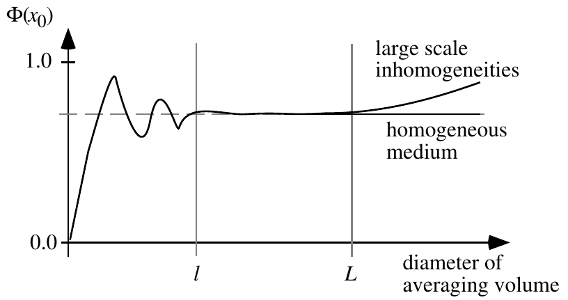
\includegraphics[width=0.5\textwidth,center]{model-rev2}
\caption{شماتیک تغییرات خواص ماکروسکوپیک نسبت به شعاع حجم نماینده}
\label{fig:2rev2}
\end{figure}
%----------------------------------------------------------------------------------------ی
%----------------------------------------------------------------------------------------ی
%                                    قسمت دوم - معادلات
%----------------------------------------------------------------------------------------ی
%----------------------------------------------------------------------------------------ی
\section{معادلات}
%----------------------------------------۲-۱: قانون پایستگی جرم-----------------------------ی
\subsection{قانون پایستگی جرم}
قانون پایستگی جرم برای هر یک از فازها در محیط متخلخل به صورت معادله \ref‌فر{eq:2cons} بیان می‌شود.
\begin{equation}
\label{eq:2cons}
\frac{\partial(\phi \varrho_\alpha S_\alpha)}{\partial t} +
\nabla \cdot (\varrho_\alpha \vec{u}_\alpha) =
\varrho_\alpha q_\alpha 
\quad \alpha=w,o
\end{equation}

\begin{tight_itemize}
\item[$\phi$] 
پارامتر تخلخل که به صورت میزان حجم خالی به حجم کل در نماینده حجم تعریف می‌شود. به طور کلی این پارامتر می‌تواند تابع فشار، دما، مکان و \dots‌خ{} باشد. در این پروژه تخلخل را تابعی از مکان و به صورت قطعه قطعه ثابت\footnote{Peicewise Constant} در نظر می‌گیریم.
\item[$S$] 
پارامتر اشباع است. در واقع اشباع هر فاز برابر است با نسبت میزان حجم آن فاز به کل حجم خالی در حجم نماینده.
\item[$\varrho$] 
نماینده چگالی هر فاز است. در این پروژه فاز‌ها را تراکم‌ناپذیر فرض می‌کنیم لذا چگالی‌ها ثابت خواهند بود. 
\item[$t$] 
زمان.
\item[$\vec{u}$] 
سرعت ماکروسکوپیک هر فاز.
\item[$q$] 
ترم‌های چشمه و چاه. در این پروژه از این ترم‌ها استفاده نخواهیم کرد.
\item[$\alpha$] 
نماینده هر فاز است. در این پروژه فاز آب را با $w$ و فاز نفت را با $o$ نمایش می‌دهیم.
\end{tight_itemize}

%----------------------------------------۲-۲: قانون دارسی-----------------------------

\subsection{قانون دارسی}
در مدل‌سازی در مقیاس ماکرو‌سکوپیک به جای استفاده از قانون پایستگی اندازه‌حرکت خطی از قانون دارسی استفاده می‌شود. این قانون زمانی که عدد رینولدز کوچک‌تر از یک باشد معتبر است و برای جریان دو‌فازی به صورت معادله \ref‌فر{eq:2darcy} بیان می‌شود.
\begin{equation}
\label{eq:2darcy}
\vec{u}_\alpha = 
-\frac{\textbf{K}k_{r\alpha}}{\mu_\alpha}
\nabla \cdot (p_\alpha+\varrho_\alpha  g h) \quad \alpha = w,o 
\end{equation}

\begin{tight_itemize}
\item[$\textbf{K}$] 
تانسور تراوایی مطلق. در بسیاری از حالات برای ساده‌سازی این ماتریس را قطری در نظر می‌گیرند، اما در این پروژه تمام درایه‌ها می‌توانند در این تانسور حاضر باشند (محیط ناهمسانگرد). در حالت کلّی این تانسور می‌تواند تابع مکان، فشار و \dots‌خ{} باشد. در این پروژه فرض می‌کنیم که این تانسور در مکان به صورت قطعه قطعه ثابت باشد.   
\item[$k_r$] 
تابع تراوایی نسبی که تابعی از اشباع هر یک از فازهاست. این پارامتر وابستگی تراوایی به اشباع را مدل می‌کند. در ادامه چند مورد از منحنی‌های این تابع را معرفی خواهیم کرد. معمولا
$k_{r\alpha}/\mu_\alpha$ 
را با $\lambda_\alpha$ نمایش می‌دهند و آن را ضریب تحرک\footnote{Mobility} می‌نامند.
\item[$\mu$]
لزجت هر فاز. در این پروژه فرض می‌شود که لزجت ثابت می‌ماند. 
\item[$p$] 
فشار ماکروسکوپیک هر فاز. 
\item[$g$] 
شتاب جاذبه. 
\item[$h$]
ارتفاع نسبت به مبداء جاذبه. جهت شتاب جاذبه لزومی ندارد که در جهت محور عمودی بوده و می‌تواند دلخواه باشد. 
\end{tight_itemize}

%----------------------------------------۲-۳ معادلات تکمیل کننده-----------------------------

\subsection{معادلات تکمیل کننده}
با توجه به این‌ که فضای خالی محیط متخلخل باید توسط دو فاز حاضر پر‌شود معادله \ref‌فر{eq:2spsone} را خواهیم داشت.
\begin{equation}
\label{eq:2spsone}
S_w+S_o=1
\end{equation}

معادله مهم دیگر فشار فاز‌ها را به یکدیگر مربوط می‌سازد. همانطور که می‌دانیم به دلیل وجود پدیده کشش سطحی لزومی ندارد که در معادله دارسی  فشار فازها ($p_w$ و $p_o$) با یکدیگر برابر باشند و اختلاف آن‌ها فشار مویینگی ($p_c$) نامیده می‌شود. در حالت میکروسکوپیک فشار مویینگی تابع عوامل متعددی از جمله کشش سطحی، انحنای مرز مشترک دو سیال و \dots‌خ{} می‌باشد. اما در حالت ماکروسکوپیک فشار مویینگی را تابعی از مکان و اشباع در نظر می‌گیرند:
 $p_c = p_c(S_w,\vec{X})$ .
در این پروژه برای ساده‌تر شدن برنامه‌نویسی فر‌آیند حل عددی تابعیت فشار مویینگی نسبت به زمان و مکان را جدا از هم در نظر می‌گیریم، یعنی: 
$p_c(S_w,\vec{X})=P_d(\vec{X}) J(S_w) $ .
به علاوه فرض می‌کنیم که ضریب $P_d$ به صورت قطعه قطعه ثابت باشد. لذا معادله \ref‌فر{eq:2pc} آخرین معادله مورد نیاز برای مدل‌کردن جریان دوفازی در محیط متخلخل می‌باشد. در ادامه چند مورد از منحنی‌های $J$ را معرفی خواهیم کرد.
\begin{equation}
\label{eq:2pc}
p_o-p_w=P_d(\vec{X})J(S_w)
\end{equation}
معادلات \ref‌فر{eq:2cons}--\ref‌فر{eq:2pc} معادلات لازم برای حل مجهولات
$S_w$، $S_o$، $p_w$، $p_o$،  
$\vec{u}_w$
 و
$\vec{u}_o$
 را تشکیل می‌دهند. 
%----------------------------------------۲-۴ معادلات مناسب برای شبیه‌سازی-----------------------------
\subsection{شکل تغییر یافته معادلات، مناسب برای شبیه سازی عددی}
در این قسمت که برگرفته از \cite{mont1,hoteitn,karimi1} است، فرمی از معادلات که برای شبیه‌سازی عددی استفاده خواهیم کرد را معرفی می‌‌کنیم. در اوّلین قدم، برای ساده‌تر شدن مدلسازی جاذبه متغیر‌های پتانسیل فاز آب، نفت و مویینگی را به صورت معادلات \ref‌فر{eq:2phia} و \ref‌فر{eq:2phic} تعریف می‌کنیم:
\begin{align}
\label{eq:2phia}
&\varphi_\alpha = p_\alpha + \varrho_\alpha g h \quad \alpha=w,o\\
\label{eq:2phic}
&\varphi_c = p_c + (\varrho_o - \varrho_w ) g h 
\end{align} 

در ادامه با توجه به اینکه در هر ناحیه از محیط متخلخل امکان دارد آب هم‌زاد\footnote{Connate Water - $S_{wc}$} یا نفت مانده\footnote{Residual Oil - $S_{or}$} وجود داشته باشد، برای مدل کردن آن‌ها اشباع نرمال شده را تعریف می‌کنیم:
\begin{equation}
\label{eq:2snorm}
S=\frac{S_w-S_{wc}}{1-S_{or}-S_{wc}}
\end{equation}

حال با ترکیب معادلات \ref‌فر{eq:2cons}--\ref‌فر{eq:2snorm}، صفر قرار دادن ترم‌های $q_\alpha$ و فرض تراکم‌ناپذیری به معادلات زیر می‌رسیم:
\begin{align}
	\label{eq:2comp1}
&\nabla \cdot (\lambda\textbf{K}\nabla\varphi_w + \lambda_o\textbf{K}\nabla\varphi_c) = 0 \\
	\label{eq:2comp2}
&\phi \beta \frac{\partial S}{\partial t} -
\nabla \cdot (\lambda_w\textbf{K}\nabla\varphi_w) = 0
\end{align} 

به علاوه با ترکیب معادلات \ref‌فر{eq:2darcy}، \ref‌فر{eq:2phia} و \ref‌فر{eq:2phic} سرعت کل و سرعت آب از روابط زیر به دست می‌آیند:
\begin{align}
	\label{eq:2comp3}
&u = - \lambda\textbf{K}\nabla\varphi_w - \lambda_o\textbf{K}\nabla\varphi_c \\
	\label{eq:2comp4}
&u_w =- \lambda_w\textbf{K}\nabla\varphi_w 
\end{align}

در این معادلات $\beta$ برابر $1-S_{or}-S_{wc}$ و $\lambda$ برابر $\lambda_w +\lambda_o$ می‌باشند. هم اکنون معادلات \ref‌فر{eq:2comp1} و \ref‌فر{eq:2comp2} دو معادله را برای دو مجهول $\varphi_w$ و $S$ تشکیل می‌دهند و معادلات \ref‌فر{eq:2comp3} و \ref‌فر{eq:2comp4} سرعت‌ها را بر حسب دو متغیر $\varphi_w$ و $S$ محاسبه می‌کنند که برای اعمال شرایط مرزی لازم هستند. در این معادلات $\varphi_c$ متغیر مستقلی نیست و از \ref‌فر{eq:2pc} و \ref‌فر{eq:2phic} به دست می‌آید.
%----------------------------------------------------------------------------------------ث
%----------------------------------------------------------------------------------------ث
%                                        قسمت سوم: توابع تراوایی نسبی
%----------------------------------------------------------------------------------------ث
%----------------------------------------------------------------------------------------ث
\section{توابع تراوایی نسبی}
در این قسمت تعدادی از توابعی که برای تراوایی نسبی پیشنهاد شده‌اند را معرفی خواهیم کرد. ویژگی مشترک تمام این منحنی‌ها این است که تراوایی نسبی هر فاز باید تابعی اکیداً صعودی از اشباع همان فاز باشد. با توجه به اینکه در هر ناحیه از محیط متخلخل امکان دارد آب هم‌زاد یا نفت مانده وجود داشته باشد، معمولاً این منحنی‌ها را بر حسب اشباع نرمال شده بیان می‌کنند.

منحنی‌های استفاده شده در این پروژه در جدول \ref{tab:2kr} نمایش داده شده‌اند. در این رساله برای اشاره به هر یک از آن‌ها از نام اختصاریشان استفاده خواهد شد. مدل \lr{brooks} در \cite{brooks} معرفی شده‌است. در این معادله $\lambda$ پارامتری است که وابسته به نوع خاک است و باید عددی بزرگتر از یک باشد. مدل \lr{vang} متعلق به یک محقق نمی‌باشد. قسمتی از آن در \cite{vang} و قسمتی دیگر از آن در \cite{parker} معرفی شده‌اند. در این معادله $m$ پارامتری است که وابسته به نوع خاک است و باید عددی بین صفر تا یک باشد. منحنی‌های \lr{poly} با وجود اینکه دقت کمی نسبت به دو منحنی دیگر دارند، بسیار ساده‌تر بوده و رفتار مشابهی را نسبت به آن‌ها نشان ‌می‌دهند، لذا برای بررسی صحت کد محاسباتی مناسب می‌باشند. منحنی‌های \lr{poly} در مراجع متعددی استفاده شده‌اند. امّا شاید اوّلین آن‌ها \cite{vandujnum} باشد. مثال‌هایی از این منحنی‌ها در شکل \ref{fig:2kr} به ازای 
 $k_{rw0}=k_{ro0}=1$ 
نشان داده شده‌اند.

\begin{table}
\centering
\caption{توابع تراوایی نسبی}
\label{tab:2kr}
\begin{tabular}{|c|c|l|l|}
\hline
ردیف &نام اختصاری
 &$k_{rw}$ &$k_{ro}$  \\
\hline
۱
&\lr{brooks}
&$k_{rw0}S^{3+2\lambda}$
&$k_{ro0}(1-S)^2 (1-S^{1+2\lambda})$ \\
۲ 
&\lr{vang}
&$k_{rw0} S^{\frac{1}{2}} (1-(1-S^\frac{1}{m})^m)^2$
&$k_{ro0} (1-S)^\frac{1}{2} (1-S^\frac{1}{m})^{2m}$ \\
۳
&\lr{poly}
&$k_{rw0}S^v$
&$k_{ro0}(1-S)^v$ \\
\hline
\end{tabular}
\end{table}

\begin{figure}
 \centering
\begin{subfigure}{0.3\textwidth}
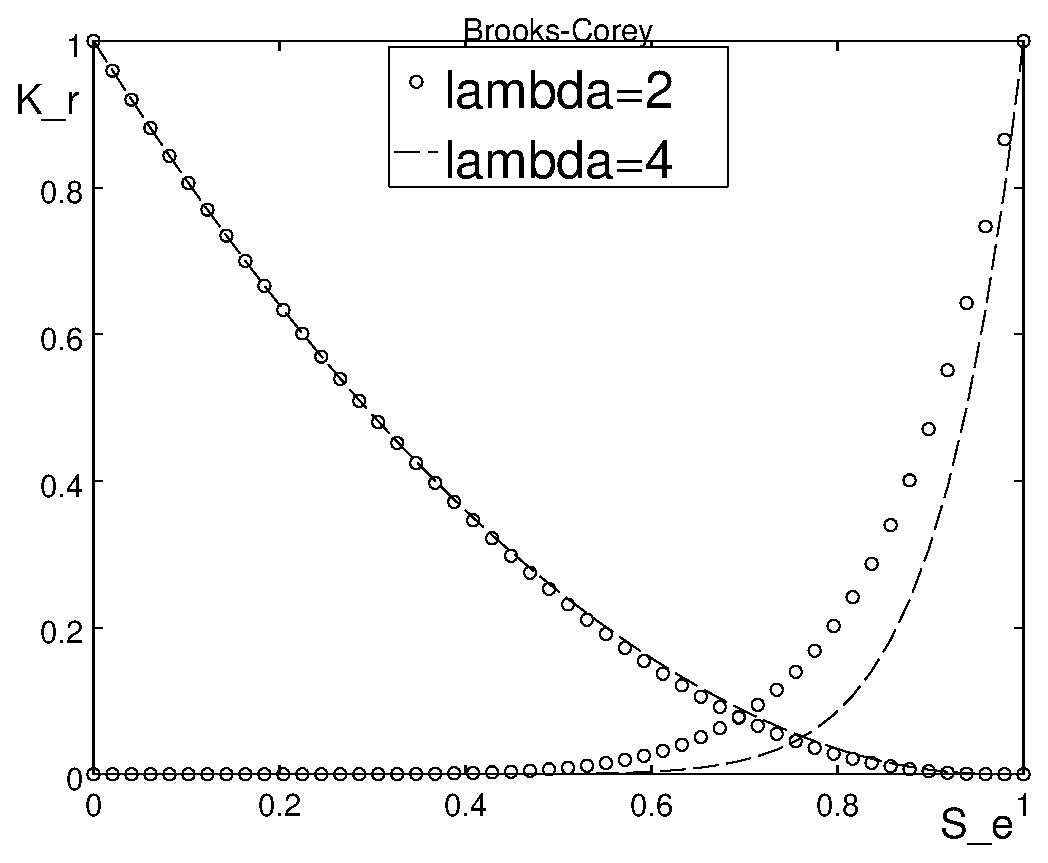
\includegraphics[width=1\linewidth]{model-kr-brooks.eps} 
\caption{منحنی‌های \text‌لاتین{brooks}}
\label{fig:2kr-brooks}
\end{subfigure}
\begin{subfigure}{0.3\textwidth}
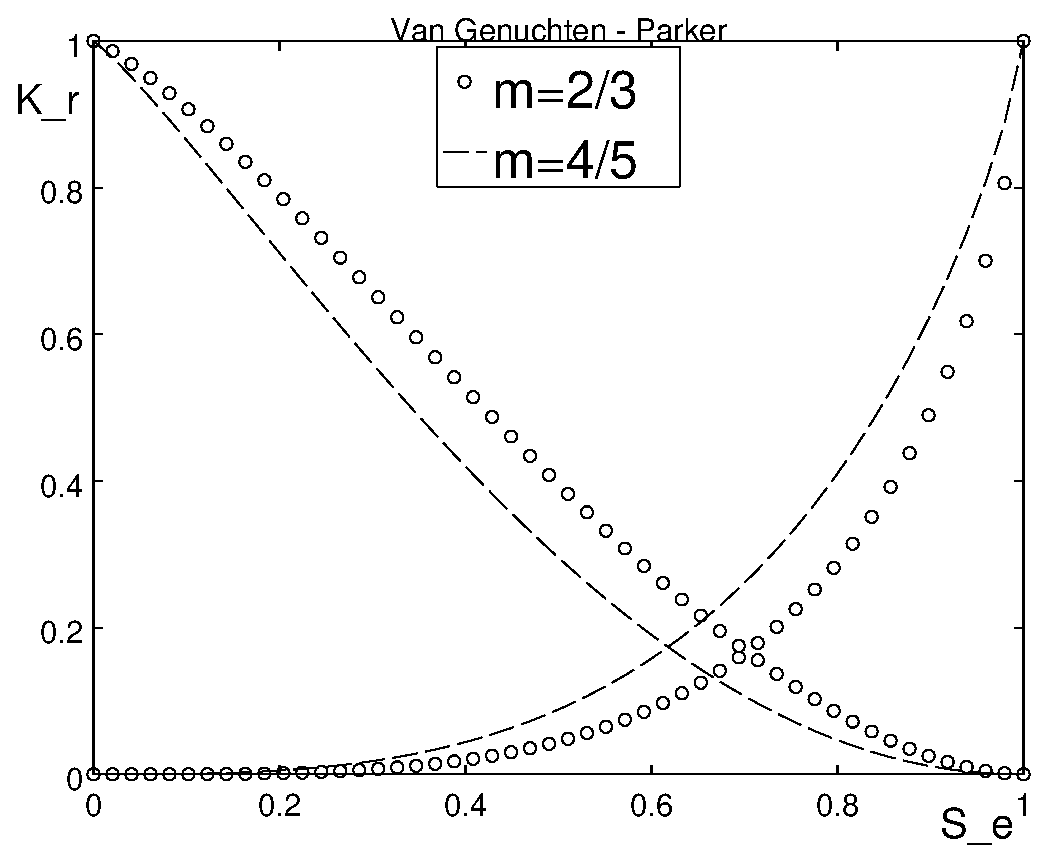
\includegraphics[width=1\linewidth]{model-kr-vang.eps}
\caption{منحنی‌های \text‌لاتین{vang}}
\label{fig:2kr-vang}
\end{subfigure}
\begin{subfigure}{.3\textwidth}
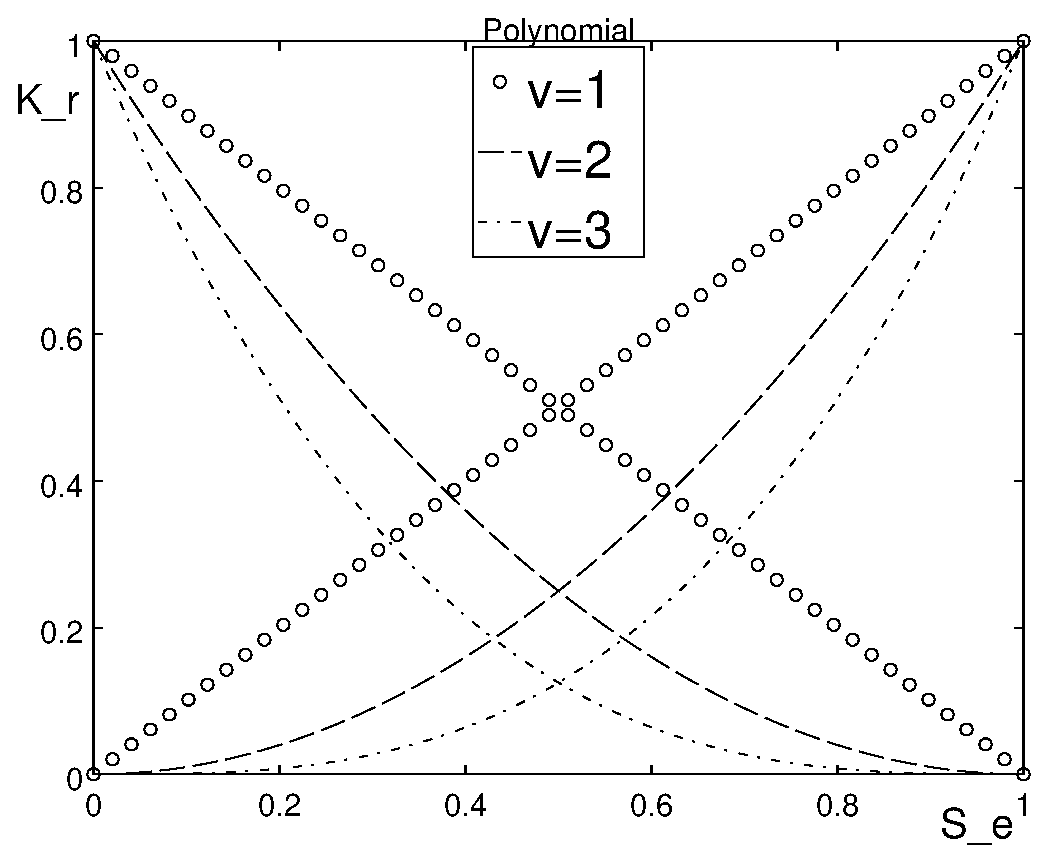
\includegraphics[width=1\linewidth, center]{model-kr-poly.eps}
\caption{منحنی‌های \text‌لاتین{poly}}
\label{fig:2kr-poly}
\end{subfigure}
\caption[مثال‌هایی از منحنی‌های تراوایی نسبی]{مثال‌هایی از منحنی‌های تراوایی نسبی به ازای $k_{rw0}=k_{ro0}=1$} 
\label{fig:2kr}
\end{figure}
%----------------------------------------------------------------------------------------ی
%----------------------------------------------------------------------------------------ی
%                                        قسمت چهارم: توابع فشار مویینگی
%----------------------------------------------------------------------------------------ی
%----------------------------------------------------------------------------------------ی
\section{توابع فشار مویینگی}
در این قسمت توابع فشار مویینگی ‌ $J$ استفاده شده را بیان خواهیم کرد. این توابع در جدول \ref{tab:2j} معرفی شده‌اند. در شکل \ref{fig:2j} نیز منحنی آن‌ها رسم شده‌اند. اگر در این منحنی‌ها $J(0) \neq 0$ به مقدار $J(0)$ فشار ورودی\footnote{Entry Pressure} می‌گویند. برای مثال منحنی \lr{brooks} دارای فشار ورودی است.


\begin{figure}[h]
\begin{subfigure}{0.3\textwidth}
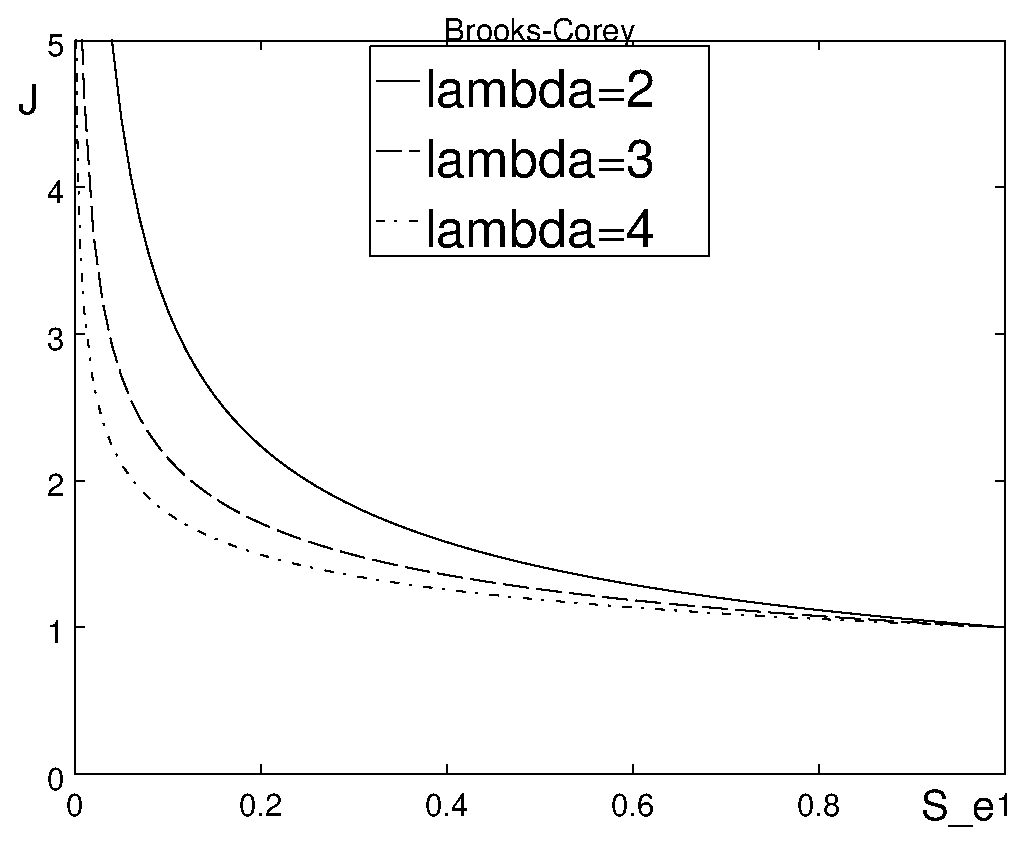
\includegraphics[width=1\linewidth]{model-j-brooks.eps} 
\caption{منحنی‌های \text‌لاتین{brooks}}
\label{fig:2j-brooks}
\end{subfigure}
\begin{subfigure}{0.3\textwidth}
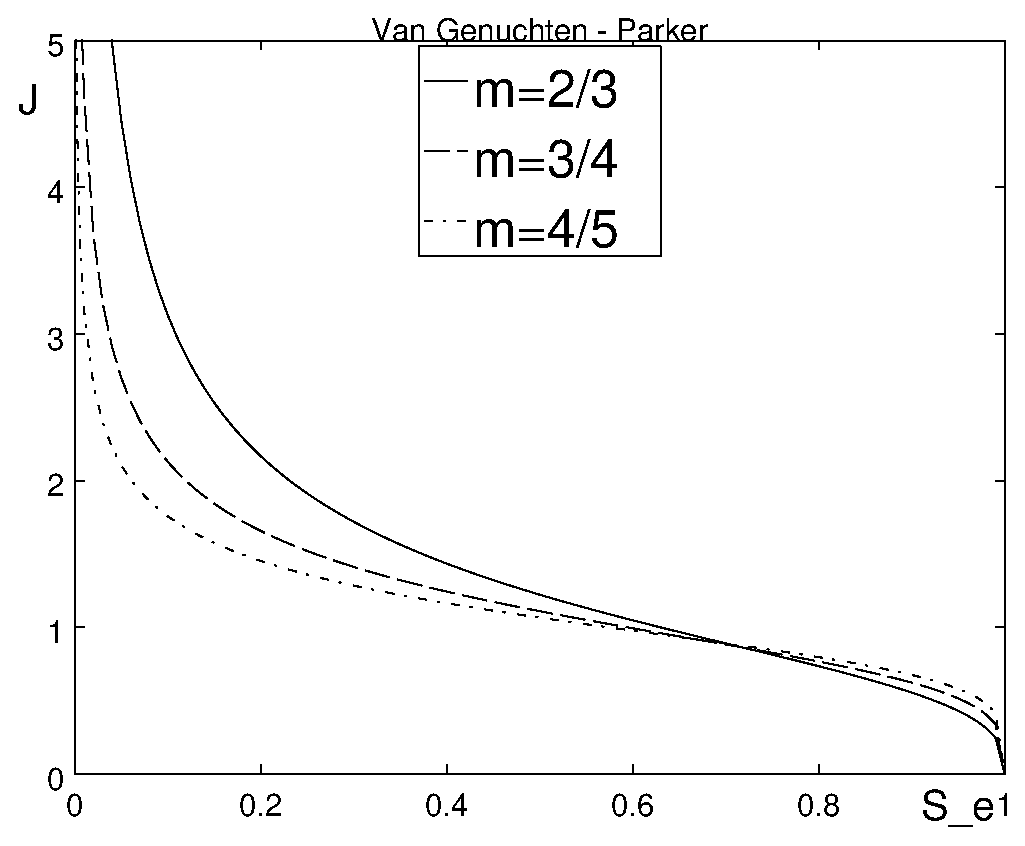
\includegraphics[width=1\linewidth]{model-j-vang.eps}
\caption{منحنی‌های \text‌لاتین{vang}}
\label{fig:2j-vang}
\end{subfigure}
\begin{subfigure}{0.3\textwidth}
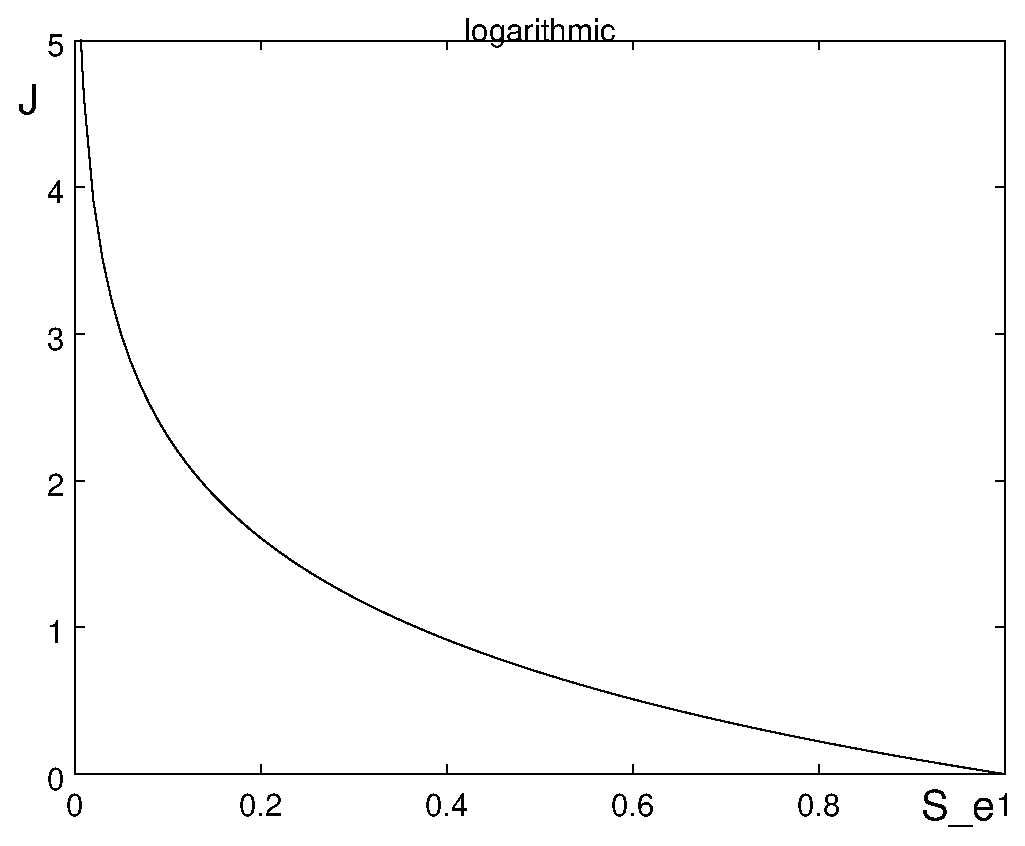
\includegraphics[width=1\linewidth, center]{model-j-log.eps}
\caption{منحنی‌ \text‌لاتین{log}}
\label{fig:2j-log}
\end{subfigure} 
\caption{منحنی‌های $J$ برای فشار مویینگی}
\label{fig:2j}
\end{figure}

\begin{table}
\centering
\caption{توابع $J$ برای فشار مویینگی}
\label{tab:2j}
\begin{tabular}{|c|c|l|l|}
\hline
ردیف &نام اختصاری
 &$J(S)$  &$J^{-1}(y)$\\
\hline
۱
&\lr{brooks}
&$S^{-\frac{1}{\lambda}}$
&$y^{-\lambda}$ \\
۲ 
&\lr{vang}
&$( S^{-\frac{1}{m}} -1 )^{1-m}$
&$(1+y^{ \frac{1}{1-m} }) ^ {-m}$ \\
۳
&\lr{log}
&$-ln(S)$
&$exp(-y)$ \\
۴
&\lr{poly}
&$(1-S)^w$
&$1-y^{1/w}$ \\
\hline
\end{tabular}
\end{table}

همانطور که در شکل \ref{fig:2j} مشاهده می‌کنید بیشتر منحنی‌های $J$ در صفر به سمت بی‌نهایت می‌روند. با توجه به معادله \ref‌فر{eq:2comp1} اگر از این منحنی‌ها برای تخمین فشار مویینگی استفاده کنیم، به مشکل برخواهیم خورد. چرا که مقدار بی‌نهایت در این معادله ظاهر خواهد شد. در این پروژه برای رفع این مشکل بجای استفاده از منحنی‌های اصلی از منحنی‌های قطع شده\footnote{$J_{trunc}$} که در معادله \ref‌فر{eq:2trunc} معرفی شده‌اند استفاده می‌کنیم. منحنی‌های قطع شده در بازه $[\epsilon \quad \infty]$ همان مقدار توابع عادی را دارند ولی در بازه $[0\quad  \epsilon]$ مقدار ثابتی خواهند داشت. متغیر $\epsilon$ به گونه‌ای انتخاب می‌شود که $J_{trunc}(0)$ مقدار معقولی داشته باشد. این روش مطابق با مراجع \cite{mont1,karimi1} می‌باشد.
\begin{equation}
\label{eq:2trunc}
J_{trunc}(S)= 
\begin{cases}
J(\epsilon) &S<\epsilon \\
J(S) &S \geq \epsilon
\end{cases}
\end{equation}

البته راه‌های دیگری نیز برای رفع این مشکل وجود دارد. یکی از آن‌ها استفاده از فرمولاسیونی متفاوت امّا معادل با معادلات  \ref‌فر{eq:2comp1}--\ref‌فر{eq:2comp4}  برای شبیه‌سازی عددی است. برای مثال در \cite{basthabil} استفاده از فشار جهانی\footnote{Global Pressure} به جای فشار مویینگی پیشنهاد شده‌است.
%----------------------------------------------------------------------------------------ی
%----------------------------------------------------------------------------------------ی
%                                        قسمت پنجم: شرایط مرزی
%----------------------------------------------------------------------------------------ی
%----------------------------------------------------------------------------------------ی
\section{شرایط مرزی و اولیه}
%----------------------------------------شرایط اولّیه-----------------------------
\subsection{شرط اولیه}
زمانی که فاز‌ها را تراکم‌ناپذیر فرض کنیم فقط نیاز به شرایط اولّیه برای اشباع داریم. لذا شرط اولّیه باید به صورت معادله \ref‌فر{eq:2ini} باشد.
\begin{equation}
\label{eq:2ini}
S(\vec{X},t=0)=S_{0}(\vec{X})
\end{equation} 
%----------------------------------------مرزهای خارجی-----------------------------ی
\subsection{مرز‌های خارجی}
برای حل معادلات \ref‌فر{eq:2comp2}، \ref‌فر{eq:2comp1} نیاز به اعمال شرایط مرزی مناسب برای مرزهای خارجی داریم. به این منظور مرز خارجی هندسه را مانند شکل \ref{fig:2bndout} به نواحی مختلف تقسیم می‌کنیم و در ناحیه یک شرط برای متغیر $\varphi_w$ و یک شرط برای متغیر  $S$ اعمال می‌کنیم. شروط استفاده شده باید توجیه فیزیکی داشته باشند، در غیر اینصورت امکان دارد که معادله جواب نداشته باشد. در معادله \ref‌فر{eq:2bndout} شروطی که در این پروژه از آن‌ها استفاده کرده‌ایم آمده‌اند:
\begin{figure}
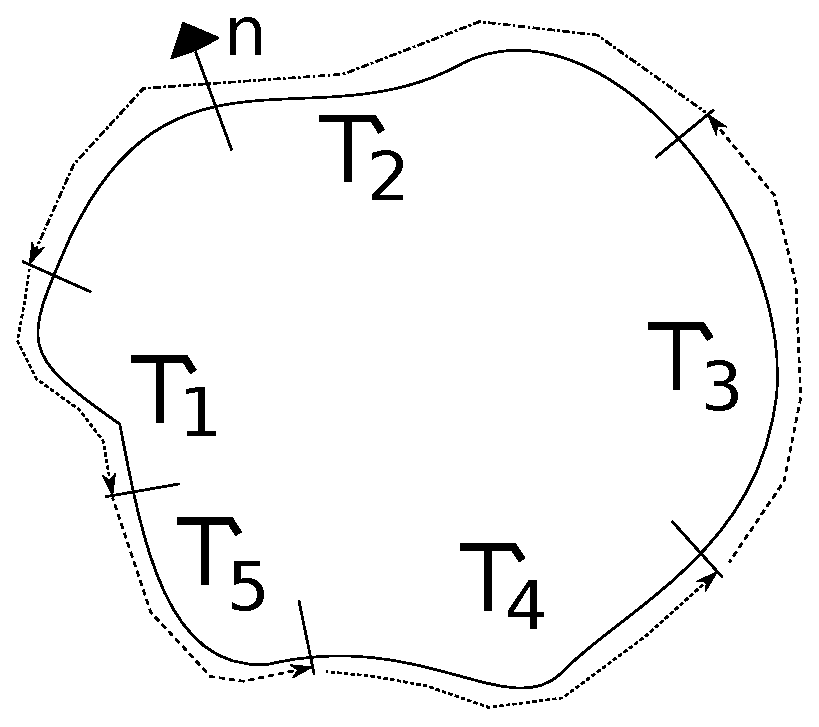
\includegraphics[width=0.4\textwidth,center]{model-bnd-out.eps}
\caption{تقسیم مرز خارجی به نواحی مختلف برای اعمال شرایط مرزی.}
\label{fig:2bndout}
\end{figure}
%-----
\begin{equation}
\label{eq:2bndout}
\begin{aligned}
&u \cdot \vec{n}
= u_N(\vec{X}) \quad 
&\vec{X} \in \Gamma_{\varphi N} \\
&\varphi_w = \varphi_D( \vec{X} ) \quad 
&\vec{X} \in \Gamma_{\varphi D} \\
&\nabla p_c \cdot \vec{n} = 0 \quad 
&\vec{X} \in \Gamma_{SN} \\
&S = S_D(\vec{X}) \quad 
&\vec{X} \in \Gamma_{SD} 
\end{aligned}
\end{equation}
%---
\begin{tight_itemize}
\item[$u_N$]
مقدار سرعت تعیین شده کل برای شرط مرزی نیومن. 
\item[$\varphi_D$] 
مقدار پتانسیل فاز آب تعیین شده بر روی مرز دیریشله.
\item[$S_{D}$] 
مقدار اشباع نرمال تعیین شده بر روی مرز دیریشله.
\item[$\Gamma_{\varphi N}$] 
مرز نیومن برای متغیر پتانسیل آب. در مرزهایی که این نوع شرط مرزی بر آن‌ها اعمال می‌شود، مقدار کل شار عبوری (آب بعلاوه نفت) بر واحد سطح باید ثابت و برابر مقدار $u_N$ باشد. این شرط مرزی برای مرز‌هایی که تزریق از آن‌ها انجام می‌شود مناسب است.
\item[$\Gamma_{\varphi D}$] 
مرز دیریشله برای متغیر پتانسیل آب. در این نوع شرط مرزی مقدار $\varphi_w$ باید ثابت و برابر $\varphi_{D}$ باشد. این نوع شرط مرزی برای مرزهایی که برداشت از آن‌ها انجام می‌شود مناسب می‌باشد. دقت شود که اگر در مسئله‌ای این شرط برای هیچ‌کدام از مرز‌ها وجود نداشته باشد، \emph{مسئله جواب نخواهد داشت}.
\item[$\Gamma_{SN}$]  
مرز نیومن برای متغیر اشباع نرمال. در این شرط مرزی گرادیان فشار مویینگی نباید مؤلفه‌ای در راستای عمود بر مرز داشته باشد. در حالتی که جاذبه وجود نداشته باشد، این صرفاً به این معنی‌ است که نسبت 
$\frac{u_w}{u_o}$ در محل مرز برابر $\frac{\lambda_w}{\lambda_o}$  
می‌باشد. دقت کنید در حالتی که جاذبه وجود داشته باشد این شرط، شرطی قابل قبول از نظر فیزیکی خواهد بود، امّا نمی‌توان آن را با شرط 
$\nabla \varphi_c \cdot \vec n = 0$
جایگزین کرد. چرا که با استفاده از قاعده زنجیری و معادله \ref‌فر{eq:2phic} این شرط به این معنی خواهد بود که:
$\nabla S \cdot \vec n= \left( P_d\frac{\partial J(S)}{\partial S} \right)^{-1} (\varrho_o - \varrho_w)g \nabla h \cdot \vec n  $
و این یعنی متغیر اشباع باید در راستای عمود بر مرز تغییر کند. این در حالی است که اگر جبهه آب به مرز نرسیده باشد نباید چنین اتفاقی رخ دهد و اشباع باید در همسایگی مرز صفر باشد. لذا این شرط از نظر فیزیکی قابل قبول نیست. شرط مرزی نیومن برای اشباع  برای مرز‌های برداشت مناسب است.
\item[$\Gamma_{SD}$] 
مرز دیریشله برای متغیر اشباع نرمال. در این نوع شرط مرزی متغیر اشباع ثابت می‌ماند. این نوع شرط مرزی برای نواحی تزریق مناسب است. 
\end{tight_itemize}

یک شرط مرزی متداول که در شبیه‌سازی‌ها از آن استفاده خواهیم کرد، مرز نفوذناپذیر است. این نوع شرط مرزی ترکیب $\Gamma_{SN}$ و $\Gamma_{\varphi N}$ با مقدار $u_N = 0$ می‌باشد. چون هیچ شاری از این مرز عبور نمی‌کند، اعمال آن در روش حجم محدود که در فصل \ref{ch:fasl3} به آن اشاره خواهیم کرد، معادل با در نظر نگرفتن آن است. نکته دیگر این است که روش عددی ما فقط قادر است مسائلی را مدل کند که در آن‌ها از بین دوناحیه شرط مرزی که مجاور یکدیگر هستند حتماً یکی نفوذناپذیر باشد. برای مثال در شکل \ref{fig:2bndout} اگر مرز‌های 
$\Gamma_2$ و $\Gamma_4$ 
نفوذناپذیر نباشند،‌ 
$\Gamma_1$، $\Gamma_3$ و  $\Gamma_5$
باید حتماً نفوذناپذیر باشند.
%----------------------------------------مرزهای داخلی-----------------------------
\subsection{مرز‌های داخلی}
\label{ch:253}
همانطور که در هنگام معرفی معادله دارسی اشاره کردیم، خواص محیط متخلخل در این پروژه به صورت قطعه قطعه ثابت تغییر می‌کنند. هر قسمت از محیط متخلخل با خواص ثابت و متفاوت با دیگر قسمت‌ها را یک ناحیه می‌نامیم. در شکل \ref{fig:2bndin} دو ناحیه مجاور 
$\Omega^{I}$
و
$\Omega^{II}$
و مرز مشترک آن‌ها به نام 
$\Gamma$
 نمایش داده شده‌است.
 بنا به \cite{basthabil,vandujnum} شرایط خاصی باید بین مرز هر دو ناحیه وجود داشته باشد. به صورت سرانگشتی می‌توان این شرایط را پیوستگی فشار و شار هر دو فاز روی مرز‌های داخلی نامید.
\begin{figure}
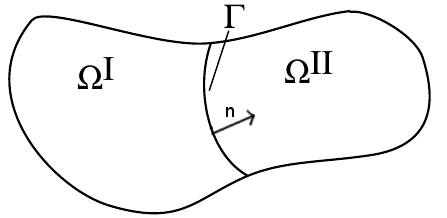
\includegraphics[width=0.6\textwidth,center]{model-bnd-in.png}
\caption{دو ناحیه مجاور یکدیگر و مرز مشترک}
\label{fig:2bndin}
\end{figure}
شروط مربوط به پیوستگی شار‌ها و فشار فاز آب در معادله \ref‌فر{eq:2bndin} نشان‌ داده شده‌اند. این شرایط باید بر روی مرز $\Gamma$ برقرار باشند. در این معادلات بالاوند $I$ یا $II$ به معنای حد مقدار ذکر شده روی مرز مشترک در طرف ناحیه $\Omega^{I}$ یا $\Omega^{II}$ است و $\vec n$ بردار نرمال مرز مشترک است. همانطور که در فصل \ref{ch:fasl3} خواهید دید، برقرار کردن این شروط کار دشواری نخواهد بود و روش عددی استفاده شده در این پروژه، بدون نیاز به استفاده از تدابیر اضافی آن‌ها را برقرار خواهد کرد. 
\begin{equation}
\label{eq:2bndin}
\vec{u}^I \cdot \vec n = \vec{u}^{II} \cdot \vec n, \quad
\vec{u}_w^I \cdot \vec n = \vec{u}_w^{II} \cdot \vec n, \quad
\varphi_w^I = \varphi_w^{II} 
\end{equation} 

پیوستگی فشار فاز نفت در قالب پیوستگی فشار مویینگی ظاهر خواهد شد. اما به دلیل وجود پدیده فشار ورودی در منحنی‌های فشار مویینگی \text‌لاتین{brooks} امکان پیوستگی فشار مویینگی برای بعضی از مقادیر اشباع در این منحنی وجود ندارد. به علاوه استفاده از منحنی‌های قطع شده نیز مشکل مشابهی را ایجاد می‌کند، لذا شرط مرزی مربوط به فشار مویینگی وابسته به منحنی استفاده شده برای فشار مویینگی خواهد بود. لذا این شرط را برای سه حالت مختلف بیان خواهیم کرد.
\begin{tight_enumerate}
\item $\lim_{S\to0}J(S)=\infty$ و $J(1)=0 $ این حالت را \lr{cc} می‌نامیم.
\item $\lim_{S\to0}J(S)\neq\infty$ و $J(1)=0 $ این حالت را \lr{dc} می‌نامیم.
\item $\lim_{S\to0}J(S)=\infty$ و $J(1) > 0$ این حالت را \lr{cd} می‌نامیم.
\end{tight_enumerate}

در هر یکی از این حالات یکی از محیط‌ها ارباب‌\footnote{Master} و دیگری برده\footnote{Slave} نام خواهد گرفت و اشباع ناحیه برده بر حسب ناحیه ارباب محاسبه خواهد شد. در حالتی نیز که در یک نقطه چند ناحیه با هم برخورد کنند باز یکی از آن‌ها ارباب خواهد بود و اشباع دیگر نواحی از اشباع این ناحیه به دست‌ خواهد آمد.
%------------منحنی cc-----
%-------------------------ی
\subsection*{حالت \text‌لاتین{cc}}
روش مدل‌کردن این حالت از \cite{mont2} برگرفته شده‌است. در این حالت فشار مویینگی می‌تواند برای تمام مقادیر اشباع ‌پیوسته باشد. فقط کافی است که رابطه \ref‌فر{eq:2ss} بین اشباع در دو طرف مرز برقرار باشد. به علاوه در این حالت انتخاب محیط‌های ارباب و برده اختیاری است.
\begin{equation}
\begin{aligned}
\label{eq:2ss}
&P_d^{slave}J(S_{slave}) = P_d^{master}J(S_{master})
\Leftrightarrow \\
&S_{slave} = J^{-1}(RJ(S_{master})) \quad R=\frac{P_d^{master}}{P_d^{slave}}
\end{aligned}
\end{equation}
جدول \ref{eq:2ss} مقادیر تابع $J^{-1}(RJ(S_{master}))$ را برای توابع $J$ معرفی شده نشان می‌دهد. با اینکه در این جدول مقدار این تابع را برای تمامی توابع $ٓJ$ محاسبه کرده‌ایم شرط \ref‌فر{eq:2ss} به عنوان شرط مرزی فقط برای مدل‌های \text‌لاتین{log} و \text‌لاتین{vang} صدق می‌کند چرا که فقط آن‌ها دارای شرایط \text‌لاتین{cc} می‌باشند. در شکل \ref{fig:2ss} می‌توانید مقدار $S_{slave}$ بر حسب $S_{master}$ را برای این مدل‌ها مشاهده کنید. 
\begin{table}
\centering
\caption{تابع $J^{-1}(RJ(S_{master}))$ برای مدل‌های متفاوت $J$}
\label{tab:2ss}
\begin{tabular}{|c|c|l|}
\hline
ردیف &مدل 
&$J^{-1}(RJ(S_{master}))$  \\
\hline
۱
&\lr{brooks}
&$R^{-\lambda}S$ \\
۲ 
&\lr{vang}
&$\left[ R^\frac{1}{1-m} (S^{-\frac{1}{m}} - 1) + 1 \right] ^ {-m} $ \\
۳
&\lr{log}
&$S^R$ \\
۴
&\lr{poly}
&$1-R^{\frac{1}{w}}(1-S)$ \\
\hline
\end{tabular}
\end{table}

%------------منحنی dc-----
%-------------------------ی
\subsection*{حالت \text‌لاتین{dc}}
در این حالت سعی می‌کنیم فرمولی که برای $S_{slave}$ در حالت منحنی‌های قطع شده ارائه می‌دهیم، شباهت زیادی به حالت قطع نشده داشته باشد. به همین منظور یک منحنی قطع شده را مانند شکل \ref{fig:2schss-dc} در نظر بگیرید. برای این حالت ناحیه ارباب ناحیه‌ای است که فشار مویینگی بیشتری دارد. مقدار $S^*_l$ را همانند این شکل \ref{fig:2schss-dc} و فرمول \ref‌فر{eq:2sl} تعریف می‌کنیم.
\begin{figure}
\begin{subfigure}{0.5\textwidth}
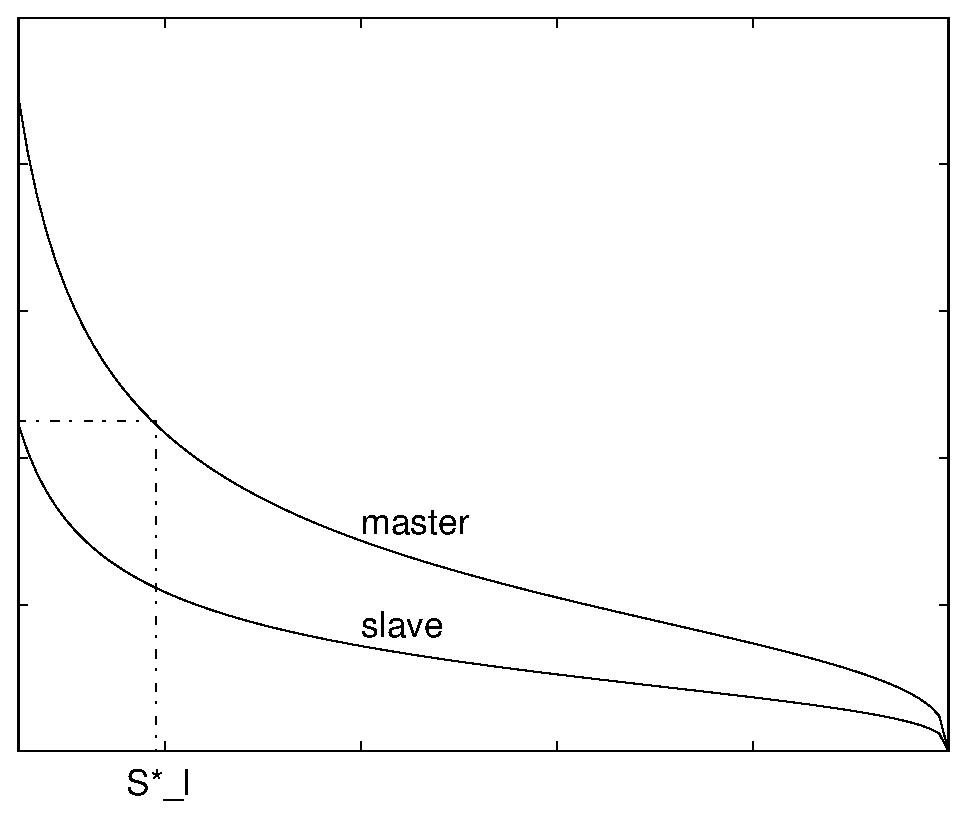
\includegraphics[width=0.8\linewidth,center]{model-ss-concept-dc.eps} 
\caption{حالت \lr{dc}}
\label{fig:2schss-dc}
\end{subfigure}
\begin{subfigure}{0.5\textwidth}
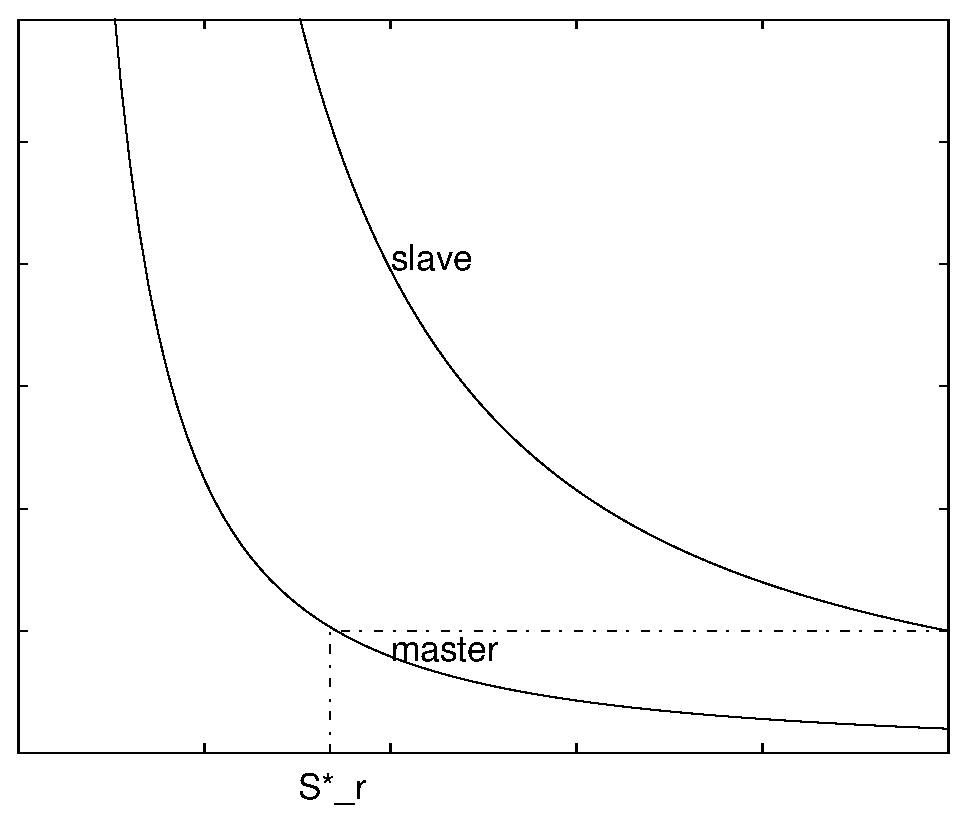
\includegraphics[width=0.8\linewidth,center]{model-ss-concept-cd.eps}
\caption{حالت \lr{cd}}
\label{fig:2schss-cd}
\end{subfigure}
\caption{شماتیک منحنی‌های فشار مویینگی برای دو محیط مجاور.}
\label{fig:2schss}
\end{figure}
\begin{equation}
\label{eq:2sl}
S_l^* = J^{-1}(\frac{1}{R}J(0))
\end{equation} 
حال می‌توانیم $S_{slave}$ را به صورت فرمول \ref‌فر{eq:2ssdc} تعیین کنیم:
\begin{equation}
\label{eq:2ssdc}
S_{slave} =
\begin{cases}
J^{-1}(RJ(S_{master})) &S_{master} > S_l^* \\
0 &S_{master} \leq S_l^* \\
\end{cases}
\end{equation} 

در شکل \ref{fig:2err} اختلاف $S_{slave}$ محاسبه شده برای مدل‌های \text‌لاتین{vang} و \text‌لاتین{log} از روش‌های قطع شده و قطع نشده قابل مشاهده است. همانطور که می‌بینید این اختلاف حداکثر به ۰٫۰۱ می‌رسد و این نشانه خوبی برای تأیید روش معرفی شده است. 

%------------منحنی cd-----
%-------------------------ی
\subsection*{حالت \text‌لاتین{cd}}
روش مدل‌کردن این حالت از \cite{basthabil} برگرفته شده‌است. در این حالت ناحیه ارباب باید ناحیه‌ای انتخاب شود که کمترین فشار مویینگی را دارد. مقدار $S^*_r$ را مانند شکل \ref{fig:2schss-cd} و فرمول \ref‌فر{eq:2sr} معرفی می‌کنیم.
\begin{equation}
\label{eq:2sr}
S_r^* = J^{-1}(\frac{1}{R}J(1))
\end{equation} 
حال می‌توانیم $S_{slave}$ را به صورت فرمول \ref‌فر{eq:2sl} تعیین کنیم:
\begin{equation}
\label{eq:2sscd}
S_{slave} =
\begin{cases}
1 &S_{master} > S_r^* \\
J^{-1}(RJ(S_{master})) &S_{master} \leq S_r^* \\
\end{cases}
\end{equation} 
در شکل \ref{fig:2ss-brooks} منحنی $S_{slave}$ را برای فشار مویینگی مدل \text‌لاتین{brooks} مشاهده می‌کنید.
\begin{figure}
\begin{subfigure}{0.5\textwidth}
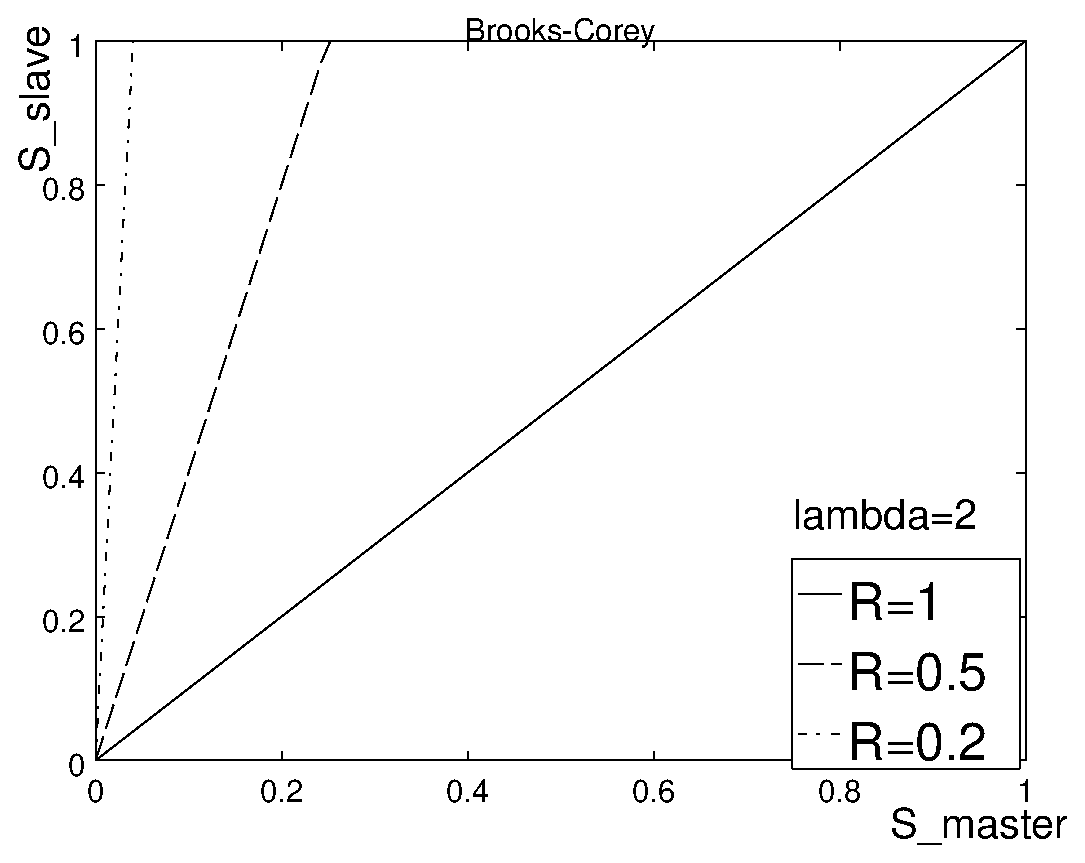
\includegraphics[width=0.9\linewidth,center]{model-ss-brooks.eps} 
\caption{مدل \text‌لاتین{brooks}}
\label{fig:2ss-brooks}
\end{subfigure}
\begin{subfigure}{0.5\textwidth}
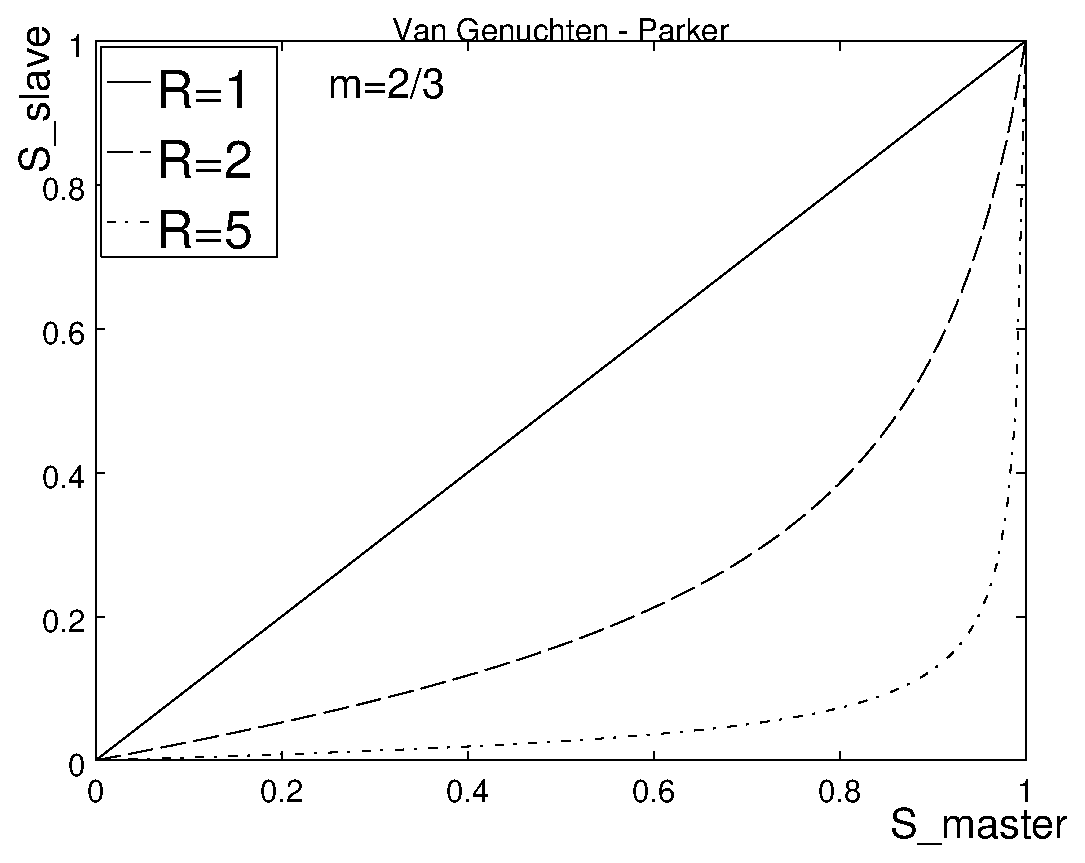
\includegraphics[width=0.9\linewidth,center]{model-ss-vang.eps} 
\caption{مدل \text‌لاتین{vang} قطع نشده}
\label{fig:2ss-vang}
\end{subfigure}
\begin{subfigure}{0.5\textwidth}
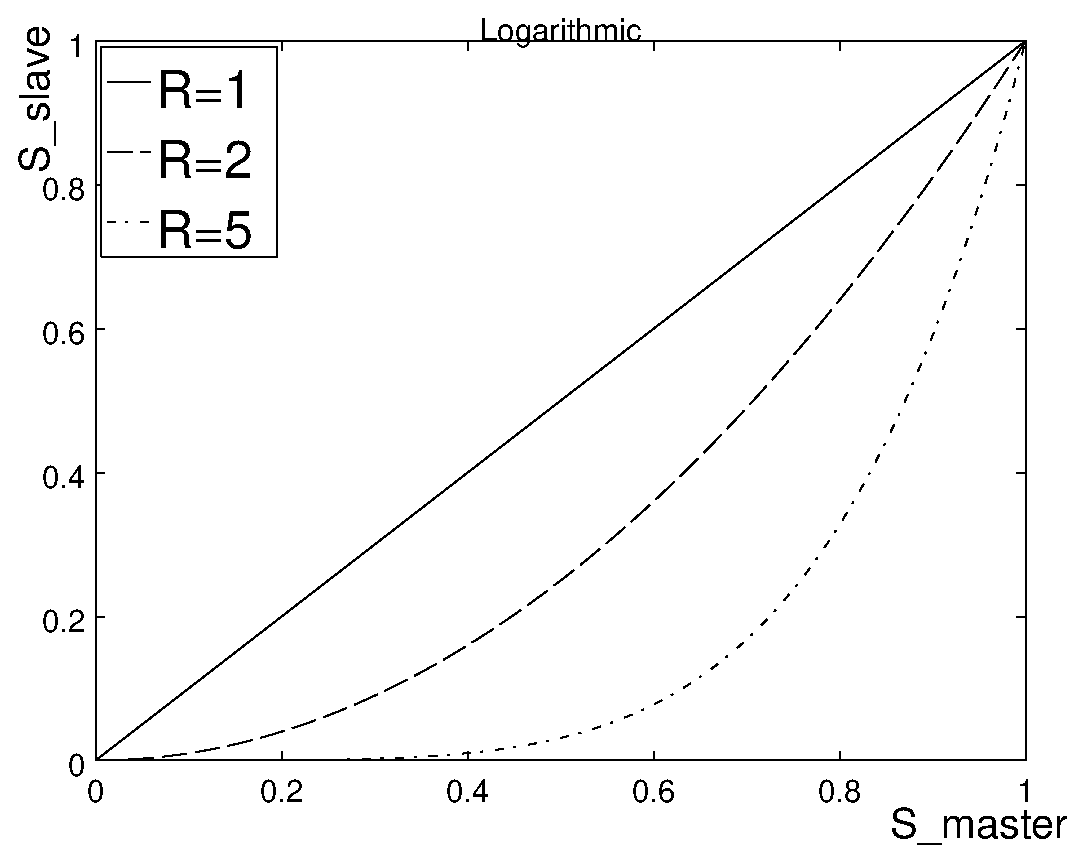
\includegraphics[width=0.9\linewidth,center]{model-ss-log.eps} 
\caption{مدل \text‌لاتین{log} قطع نشده}
\label{fig:2ss-log}
\end{subfigure}
\begin{subfigure}{0.5\textwidth}
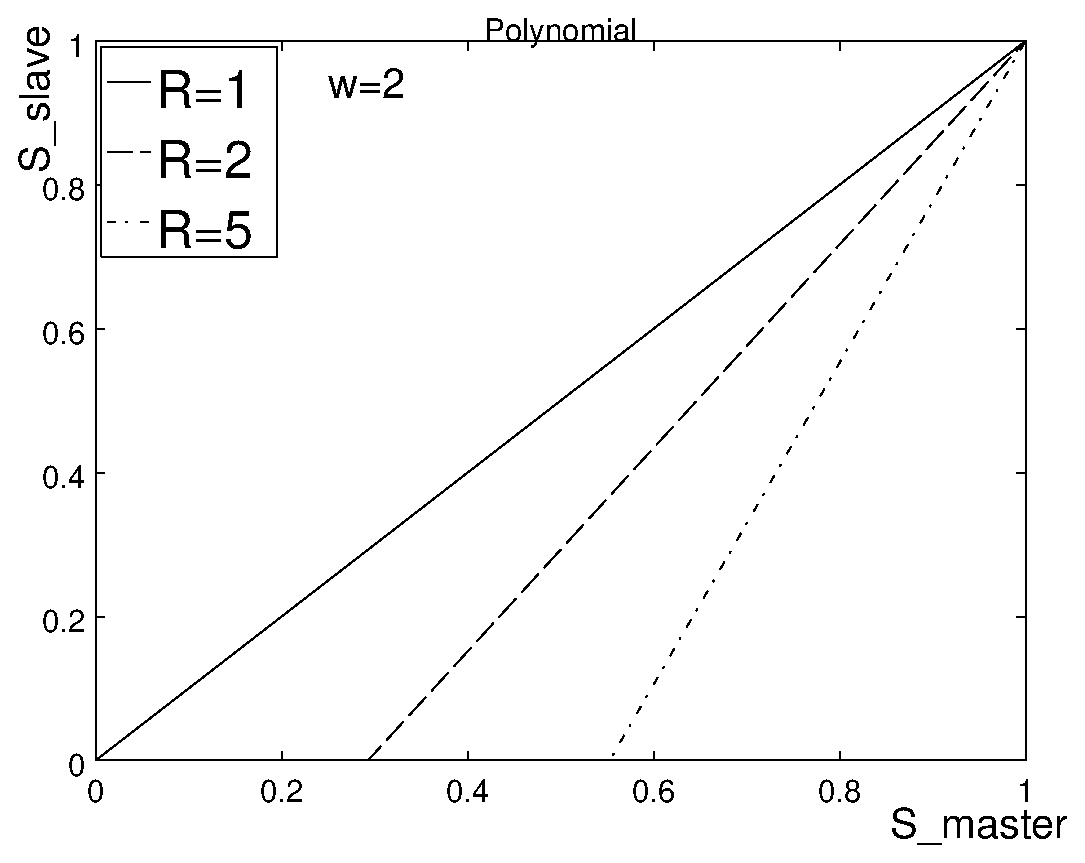
\includegraphics[width=0.9\linewidth,center]{model-ss-poly.eps} 
\caption{مدل \text‌لاتین{poly}}
\label{fig:2ss-poly}
\end{subfigure}
\caption[اشباع ناحیه برده بر حسب ناحیه ارباب]{اشباع ناحیه برده بر حسب ناحیه ارباب برای مدل‌های مختلف تابع $J$}
\label{fig:2ss}
\end{figure}
%
\begin{figure}
\begin{subfigure}{0.5\textwidth}
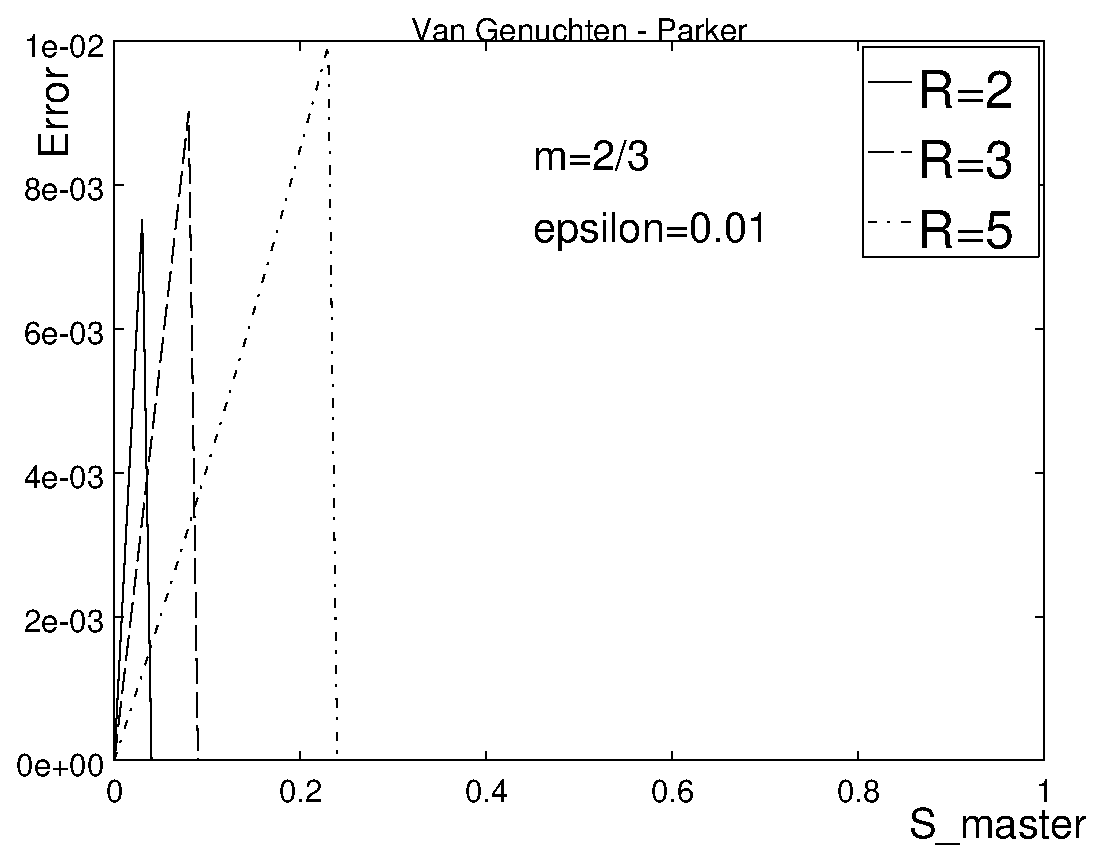
\includegraphics[width=0.9\linewidth,center]{model-sserr-vang.eps} 
\caption{مدل \text‌لاتین{vang}}
\label{fig:2err-vang}
\end{subfigure}
\begin{subfigure}{0.5\textwidth}
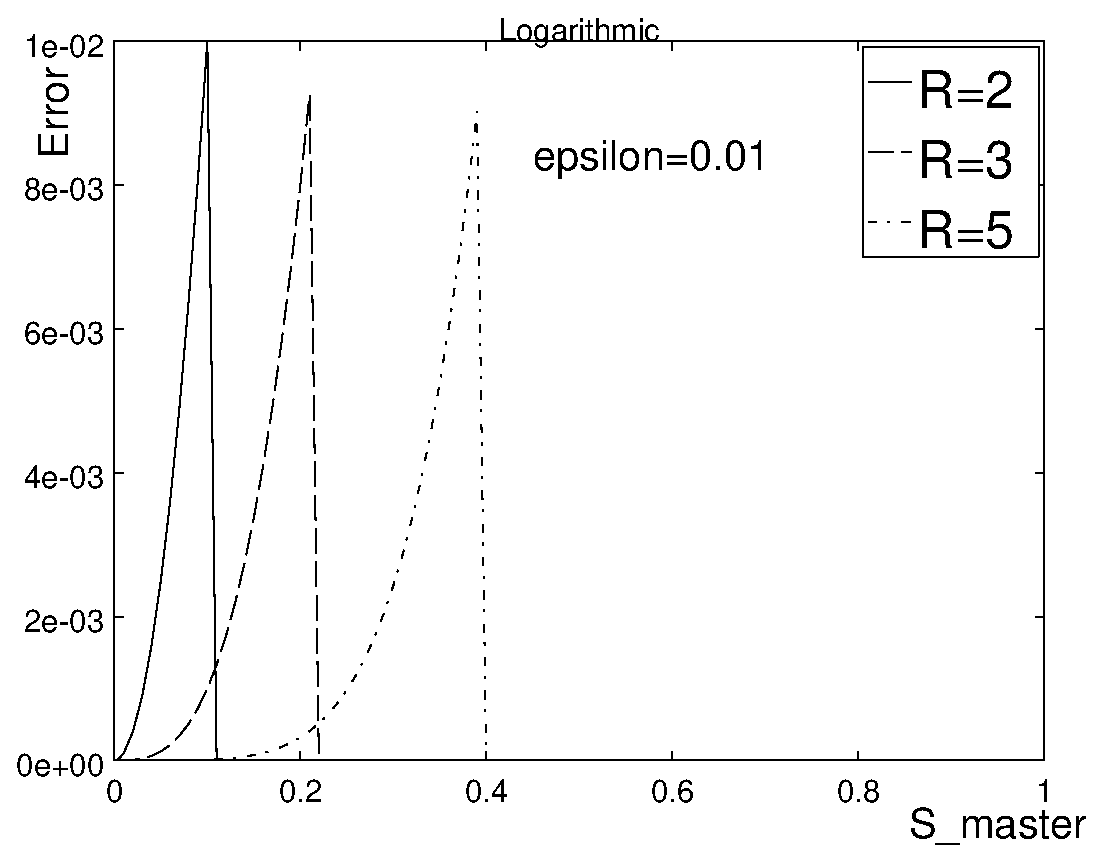
\includegraphics[width=0.9\linewidth,center]{model-sserr-log.eps} 
\caption{مدل \text‌لاتین{log}}
\label{fig:2err-log}
\end{subfigure}

\caption{تفاوت مقدار $S_{slave}$ محاسبه شده از طریق توابع $J$ قطع نشده و قطع شده}
\label{fig:2err}
\end{figure}
%----------------------------------------------------------------------------------------ی
%----------------------------------------------------------------------------------------ی
%                                       مدل ترک گسسته
%----------------------------------------------------------------------------------------
%----------------------------------------------------------------------------------------
\section{مدل ترک گسسته}
برای مدل کردن ترک‌های موجود در یک محیط متخلخل به روش ترک گسسته صرفاً کافی است که هر ترک را یک ناحیه با خواص خاص خود در محیط متخلخل در نظر بگیریم. لذا در این روش مدل کردن ترک‌ها تفاوتی با مدل کردن دیگر نواحی ماتریس محیط متخلخل ندارد. با توجه به اینکه ضخامت ترک‌ها بسیار کم است، دو روش برای مدل کردن آن‌ها وجود دارد. در روش اول شبکه محاسباتی داخل ترک با شبکه محاسباتی ماتریس هم‌بعد است. این روش هزینه محاسباتی بالایی دارد و کاربرد آن بررسی صحت روش دیگری است که معرفی خواهیم کرد. در روش دوم شبکه محاسباتی ترک بعد کمتری نسبت به شبکه محاسباتی ماتریس دارد. طبیعتاً روش عددی استفاده شده باید به گونه‌ای تعمیم داده شود که بتواند این کار را انجام دهد.

در این رساله با توجه به اینکه هند‌سه‌های دوبعدی را بررسی خواهیم کرد، روش هم‌بعد را روش ترک-دوبعدی و روش بعد کمتر را ترک-یک‌بعدی می‌نامیم. این در حالی است که در بعضی از مقالات روش ترک-دوبعدی را روش مش ریز\cite{karimi2} یا تک‌تخلخل\footnote{Single Porosity}\cite{karimi1} و روش ترک-یک‌بعدی را روش ترک گسسته می‌نامند. در شکل \ref{fig:2f} مش محاسباتی استفاده شده برای شبیه‌سازی یک ترک را برای هر یک از روش‌ها مشاهده می‌کنید.
\begin{figure}
\begin{subfigure}{0.5\textwidth}
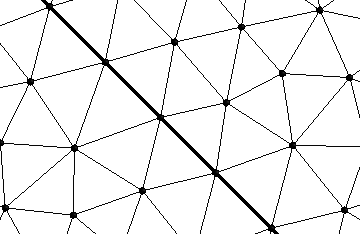
\includegraphics[width=0.9\linewidth,center]{model-mesh1.png} 
\caption{استفاده از مش یک بعدی برای ترک}
\label{fig:2f-1}
\end{subfigure}
\begin{subfigure}{0.5\textwidth}
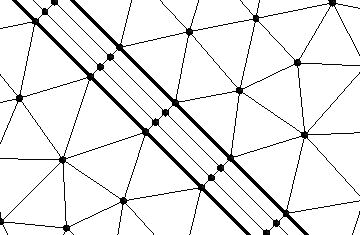
\includegraphics[width=0.9\linewidth,center]{model-mesh2.png} 
\caption{استفاده از مش دوبعدی برای تک}
\label{fig:2f-2}
\end{subfigure}

\caption{مقایسه مش استفاده شده برای حالت‌های ترک-یک‌بعدی و ترک-دوبعدی}
\label{fig:2f}
\end{figure}
